\section{Fichiers et repertoires}
\subsection{Les noms et contenus des fichiers}
\begin{frame}{Noms et contenu des fichiers}
  \begin{block}{La décomposition traditionnelle d'un nom de fichier}
    \begin{columns}
      \begin{column}{8cm}
        Deux parties séparées par un point:
        \begin{itemize}
        \item La $1\up{ère}$ partie informe sur la nature du contenu du
          fichier,
        \item La $2\up{ème}$ partie informe sur le format ou la finalité des données.
        \end{itemize}
      \end{column}
      \begin{column}{3cm}
        \begin{tabular}{|r@{}r@{}l|}
          \hline
          {\color{solarizedRed}nom}&.&{\color{solarizedGreen}extension} \\
          {\color{solarizedRed}prefix}&.&{\color{solarizedGreen}suffix} \\
          {\color{solarizedRed}description}&.&{\color{solarizedGreen}format}\\
          \hline
        \end{tabular}
      \end{column}
    \end{columns}
  \end{block}
  \begin{columns}
    \begin{column}{5.5cm}
      \begin{block}{Exemples de formats de fichiers}
        \begin{center}
          \begin{tabular}{ll}
            \hline
            Extension&Contenu\\
            \hline
            .c&Sources C\\
            .html&Document Web\\
            .pdf&Document Mis en page\\
            .txt&Texte brut\\
            .mp3&Fichier Multimedia\\
            \hline
          \end{tabular}
        \end{center}
      \end{block}
    \end{column}
    \begin{column}{5.5cm}
      \begin{block}{Exemples de noms de fichiers}
        \begin{center}
          \begin{tabular}{ll}
            \hline
            Enigmatique&Informatif\\
            \hline
            e3.c&teste\_boucle\_for.c\\
            New.pdf&2011\_IntroSys\_cours\_1.pdf\\
            toto.sh&test\_boucle\_for.sh\\
            \hline
          \end{tabular}
        \end{center}
      \end{block}
      \vrule
    \end{column}
  \end{columns}
  \begin{alertblock}{Le choix des noms des fichiers et répertoires}
    \begin{itemize}
    \item Ils doivent être choisis minutieusement pour être informatifs,
    \item Choisir un nom : réfléchir pour un gain de temps pour
      retrouver le fichier ou le répertoire concerné.
    \end{itemize}
  \end{alertblock}
\end{frame}
\subsection{Organisation des données enregistrées}
\begin{frame}{Organisation des données enregistrées}
  \begin{block}{De très nombreux fichiers et répertoires}
    \begin{columns}
      \begin{column}{.7\linewidth}
        \begin{itemize}
        \item Le nombre de fichiers enregistrés sur un disque dur peut
          aisément dépasser 100.000 fichiers,
        \item Chaque fichier est identifié par un nom,
        \item Les fichiers sont regroupés dans des répertoires et
          sous-répertoires.
        \item Chaque répertoire est identifié par un nom.
        \end{itemize}
      \end{column}%
      \begin{column}{.25\linewidth}
        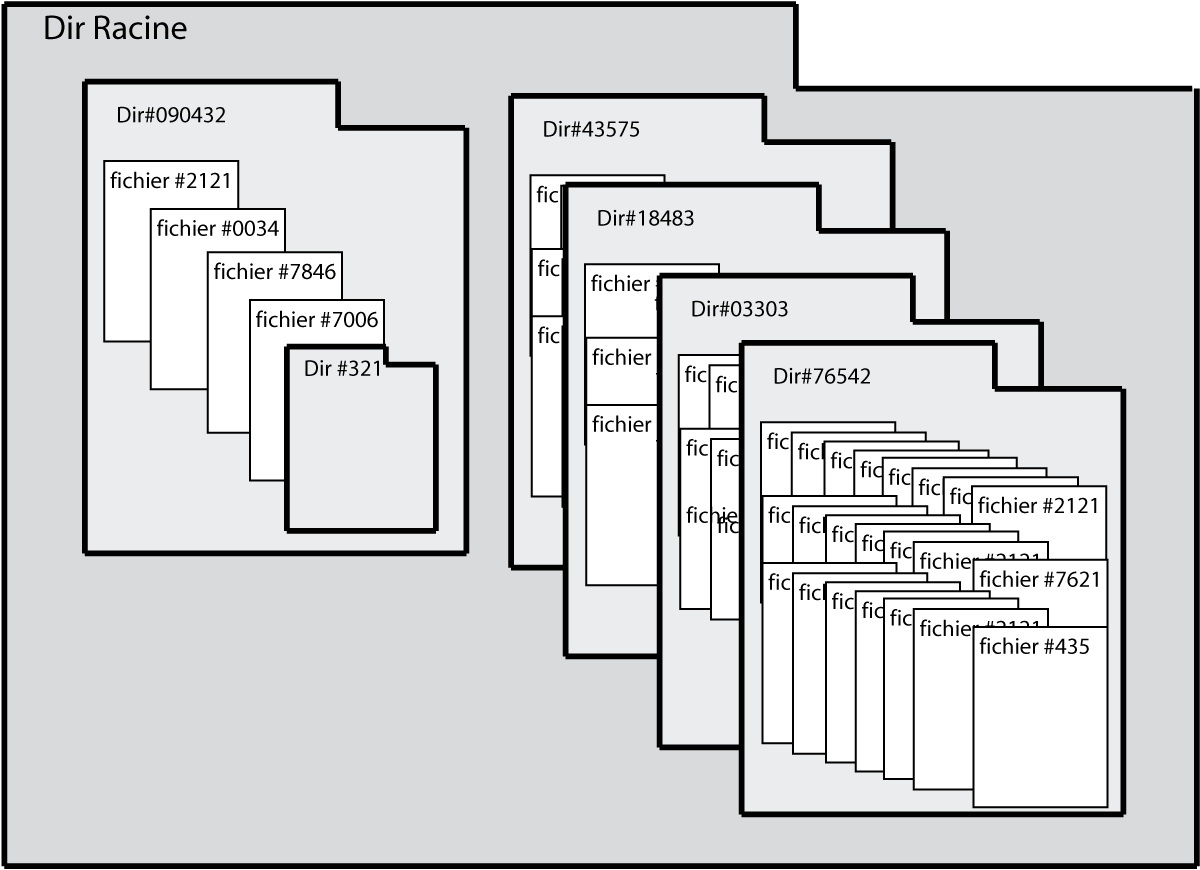
\includegraphics[width=\linewidth]{img/s02/file_system}
      \end{column}
    \end{columns}
  \end{block}
  \begin{block}{Une organisation en arborescence}
    \begin{itemize}
    \item Cette organisation arborescente permet de faciliter la
      recherche d'un fichier,
    \item Les fichiers sont regroupés par application, par thème, par
      format, par fonction, \dots \end{itemize}
  \end{block}
  \begin{alertblock}{Remarque}
    \begin{itemize}
    \item[\dialogerror] Avec tous les fichiers au même
      \textit{endroit}, il est très difficile de les lister (trop à
      lire).
    \item[\dialoginformation] Organisation \emph{hiérarchique} qui permet d'organiser les données et
      de faciliter leur accès.
    \end{itemize}
  \end{alertblock}
\end{frame}

\subsection{L'organisation arborescente}
\begin{frame}{Exemple d'arborescence Linux}
  \dirtree{%
    .1 \DTd{}\DTfcomment{Répertoire Racine ou Root Directory}.  .2
    \DTd{bin}.  .3 (\dots).  .2 \DTd{home}.  .3
    \DTd{chez\_moi}\DTfcomment{Répertoire Personnel ou User
      Directory}.  .4 \DTd{Mes\_Documents}.  .5 ListeDesCourses.txt.
    .5 Exercice\_1.sh.  .4 (\dots).  .3 \DTd{anonymous}.  .4
    LisezMoi.txt.  .4 \DTd{Telechargements}.
    % .5 Cours\_Systeme.pdf.
    .5 (\dots).  .2 (\dots).  }
  \begin{alertblock}{Les répertoires importants}
    \begin{itemize}
    \item La \textbf{racine} (\textit{Root directory}) contient tous
      les répertoires et fichiers accessibles depuis le système.
    \item Le \textbf{répertoire personnel} (\textit{User Directory} ou
      \textit{Home Directory}) est le répertoire dans lequel
      l'utilisateur peut faire ce qu'il veut (écrire, modifier,
      supprimer, installer \dots).
    \end{itemize}
  \end{alertblock}
\end{frame}
\subsection{La notion de Chemin}
\begin{frame}{La notion de Chemin}
  \begin{block}{Le chemin défini un nom unique}
    \begin{itemize}
    \item Deux fichiers ou répertoires ne peuvent pas porter le même nom si ils sont dans un même répertoire.
    \item Les noms des fichiers et répertoires différencient les caractères \textsc{Majuscules} et minuscule. Les fichiers \alert{E}ssai.txt et \alert{e}ssai.txt peuvent donc être dans le même répertoire. 
    \end{itemize}
  \end{block}
  \begin{block}{Exemples de chemins absolus}
    \dirtree{%
      .1 \DTd{}\DTfcomment{Un chemin absolu part de la racine {\color{solarizedAccent}/}}.
      .2 \DTd{home}\DTfcomment{/{\color{solarizedAccent}home/}}.
      .3 \DTd{chez\_moi}\DTfcomment{/home/{\color{solarizedAccent}chez\_moi/}}.
      .4 \DTd{Etoiles}\DTfcomment{/home/chez\_moi/{\color{solarizedAccent}Etoiles/}}.
      .5 SOLEIL.jpg\DTfcomment{/home/chez\_moi/Etoiles/{\color{solarizedAccent}SOLEIL.jpg}}.
      .5 Soleil.jpg\DTfcomment{/home/chez\_moi/Etoiles/{\color{solarizedAccent}Soleil.jpg}}.
      .4 \DTd{Systeme\_Solaire}\DTfcomment{/home/chez\_moi/{\color{solarizedAccent}Systeme\_Solaire/}}.
      .5 SOLEIL.jpg\DTfcomment{/home/chez\_moi/Systeme\_Solaire/{\color{solarizedAccent}SOLEIL.jpg}}.
    }
  \end{block}
  \begin{alertblock}{Syntaxe d'un chemin absolu}
    Le chemin \textit{absolu} d'un fichier ou d'un répertoire est unique. Il donne la liste des répertoires et sous-répertoires en partant de la racine \lin{/} (la référence \textit{absolue} de l'arborescence) jusqu'à la cible.
  \end{alertblock}
\end{frame}

\subsection{Répertoire courant et Chemins relatifs}
\begin{frame}{Répertoire courant et Chemins relatifs}
  \begin{block}{Le répertoire courant}
    \begin{itemize}
    \item Le répertoire courant est un répertoire de référence d'où sont lancées les commandes.
    \item Par défaut, le répertoire courant est le répertoire personnel de l'utilisateur,
    \item Naviguer dans l'arborescence équivaut à modifier le répertoire courant.
    \end{itemize}
  \end{block}
  \begin{block}{Exemples de chemins relatifs}
    \dirtree{%
      .1 \DTd{home}\DTfcomment{../..}.
      .2 \DTd{chez\_moi}\DTfcomment{../}.
      .3 \DTd{Etoiles}\DTfcomment{{\color{solarizedAccent}Répertoire Courant ~~./}}.
      .4 SOLEIL.jpg\DTfcomment{SOLEIL.jpg {\color{black}ou} ./SOLEIL.jpg}.
      .4 Antares.jpg\DTfcomment{Antares.jpg {\color{black}ou} ./Antares.jpg}.
      .3 \DTd{Systeme\_Solaire}\DTfcomment{../Systeme\_Solaire/}.
      .4 terre.gif\DTfcomment{../Systeme\_Solaire/terre.gif}.
    }
  \end{block}
  \begin{alertblock}{Syntaxe d'un Chemin Relatif}
    \begin{itemize}
    \item Le chemin \textit{relatif} d'un fichier ou d'un répertoire donne la liste des répertoires et sous-répertoires en partant du répertoire courant (la référence \textit{relative} dans l'arborescence) jusqu'à la cible.
    \item Il est relatif, car lorsque le répertoire courant change, le chemin relatif change.
    \end{itemize}
  \end{alertblock}
\end{frame}

%%%%%%%%%%%%%% 
\subsection{Notation spéciales}
\begin{frame}{Notation Spéciales}
  \begin{block}{Les chemins des répertoires de référence}
    \begin{columns}
      \begin{column}{6cm}
        \begin{center}
          \begin{tabular}{lr}
            \hline
            Répertoire&Notation\\
            \hline
            Répertoire Racine&\lin{/}\\
            Répertoire Personnel&\lin{\~{}}\\
            \hline
          \end{tabular}
        \end{center}
      \end{column}
      \begin{column}{6cm}
        \begin{center}
          \begin{tabular}{lr}
            \hline
            Répertoire&Notation\\
            \hline
            Répertoire Courant&\lin{.}\\
            Répertoire Parent&\lin{..}\\
            \hline
          \end{tabular}
        \end{center}
      \end{column}
    \end{columns}
  \end{block}
  \begin{alertblock}{Remarques}
    \begin{itemize}
    \item La notation \lin{\~{}} correspond à un chemin absolu. Elle est remplacée lors d'une évaluation par le chemin absolu du répertoire personnel de l'utilisateur.
    \end{itemize}
  \end{alertblock}
  \begin{block}{Exemple de chemins valides pointant le fichier cible}
    \begin{columns}
      \begin{column}{6cm}
        \dirtree{%
          .1 \DTd{}\DTfcomment{{\color{solarizedAccent}Répertoire Racine}}.
          .2 \DTd{home}.
          .3 \DTd{chez\_moi}\DTfcomment{{\color{solarizedAccent}Répertoire Personnel}}.
          .4 \DTd{Etoiles}\DTfcomment{{\color{solarizedAccent}Répertoire Courant}}.
          .5 Soleil.jpg\DTfcomment{Fichier cible}.
        }
      \end{column}
      \begin{column}{6.5cm}
        \begin{center}
          \footnotesize{
            \begin{tabular}{l}
              \hline
              Chemins Absolus\\
              \hline
              \lin{/home/chez\_moi/Etoiles/Soleil.jpg}\\
              \lin{\~{}/Etoiles/Soleil.jpg}\\
              \lin{/home/chez\_moi/../chez\_moi/Etoile/Soleil.jpg}\\
              \lin{/home/chez\_moi/../../home/chez\_moi/Etoile/Soleil.jpg}\\
              \hline
              Chemins Relatifs\\
              \hline
              \lin{Soleil.jpg}\\
              \lin{../Etoile/Soleil.jpg}\\
              \lin{../../chez\_moi/Etoile/Soleil.jpg}\\
            \end{tabular}
          }
        \end{center}
      \end{column}
    \end{columns}	
  \end{block}
\end{frame}

%%%%%%%%%%%%%% 
\subsection{Tout est fichier}
\begin{frame}{Tout est Fichier}
  \begin{block}{Gestion des fichiers}
    Lors de la création du système de fichier une table des i-nodes est créée. Celle-ci fixe le nombre maximum de fichiers.
  \end{block}
  \begin{block}{Fichiers}
    \begin{itemize}
    \item Chaque fichier est décrit comme un i-node.
    \item L'i-node contient un certain nombre de \textit{métadonnées} concernant le fichier:
      \begin{itemize}
      \item adresse sur le disque et taille du fichier en nombre d'octets,
      \item identification du propriétaire (UID et GID) et permissions (lecture, écriture et exécussion),
      \item dates de dernière modification et de dernier accès,
      \item \dots
      \end{itemize}
    \item Le nom du fichier n'est pas stocké dans son i-node!
    \end{itemize}
  \end{block}
  \begin{block}{Répertoire}
    {\color{solarizedAccent}Un répertoire est un fichier} spécial listant les références des fichiers qu'il contient sous forme de couples (nom\_du\_fichier, i-node).
  \end{block}
  \begin{block}{Fichiers spéciaux}
    Les fichiers de périphériques sont des fichiers spéciaux mis en place par le système pour assurer le lien avec un périphérique.
  \end{block}
\end{frame}
%%%%%%%%%%%%%% 
\subsection{Conventions}
\begin{frame}{Conventions}
  \begin{block}{Noms et Chemins}
    \begin{itemize}
    \item Par convention, le nom d'un fichier ou d'un répertoire est identifié avec son chemin (sauf mention contraire explicite).
    \item Par convention, un chemin peut être absolu, relatif. Il peut utiliser les notations spéciales.
    \item Par convention la notion de fichier sera comprise dans son sens large. Par exemple, le chemin d'un fichier devra être interprété sans distinction comme le chemin vers un fichier ordinaire ou comme le chemin vers un répertoire (sauf mention contraire explicite).
    \end{itemize}
  \end{block}
  \begin{block}{Commandes, options, paramètres}
    \begin{description}
    \item[Commande] c'est le nom d'un programme qui exécute une action.
    \item[Options] ce sont des paramètres optionnels. Ils peuvent être omis. L'ajout d'options modifie le comportement de la commande (le résultat). Les options sont encadrées par les caractères \lin{< options >}.
    \item[Paramètres] ce sont des arguments que la commande évalue.
    \end{description}
  \end{block}
  \begin{block}{Sources et Cible}
    \begin{description}
    \item[Source] c'est un fichier ou un répertoire utilisé en entrée d'une commande,
    \item[Cible] c'est un fichier ou un répertoire utilisé en sortie d'une commande.
    \end{description}
  \end{block}
\end{frame}
%%%%%%%%%%%%%% 
\subsection{Manipulation de l'arborescence en ligne de commande}
\begin{frame}{Manipulation de l'arborescence en ligne de commande}
  \begin{block}{Alternatives pour naviguer dans l'arborescence et manipuler les fichiers}
    \begin{columns}
      \begin{column}{6cm}
        \begin{center}
          Interface Graphique\\
          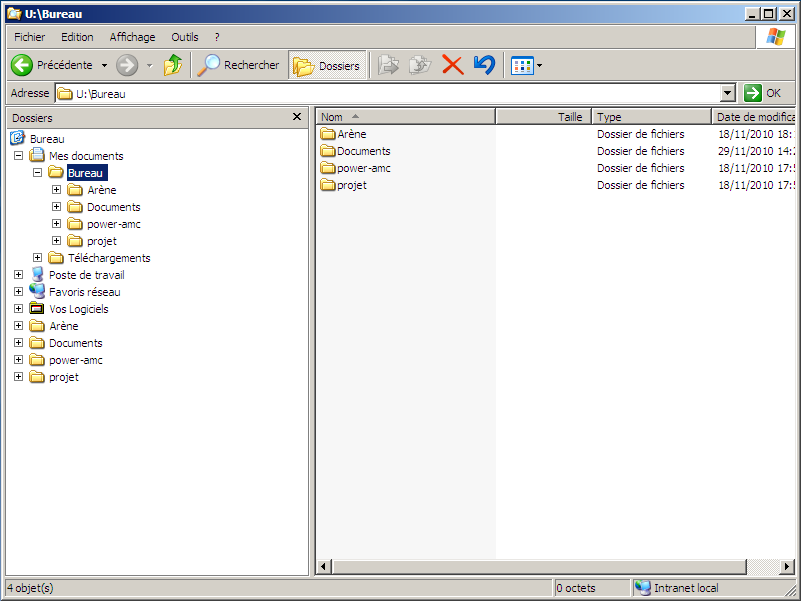
\includegraphics[height=2.5cm]{img/s02/explorer_windows.png}
        \end{center}
      \end{column}
      \begin{column}{6cm}
        \begin{center}
          Ligne de Commande\\
          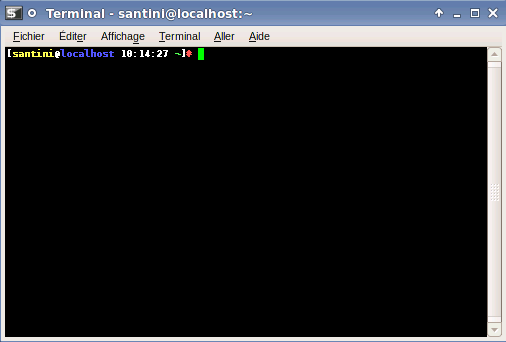
\includegraphics[height=2.5cm]{img/s02/terminal_single.png}
        \end{center}
      \end{column}
    \end{columns}
  \end{block}
  \begin{block}{Principales commandes}
    \begin{center}
      \begin{tabular}{ll}
        \hline
        Commande&Fonction principale\\
        \hline
        \lin{pwd}&Afficher le nom du répertoire courant\\
        \lin{ls}&Afficher le contenu d'un répertoire\\
        \lin{cd}&Changer de répertoire courant\\
        \lin{mkdir}&Créer un répertoire\\
        \lin{rm}&Supprimer fichier(s) ou répertoire(s) \\
        \lin{cp}&Copier fichier(s) ou répertoire(s)\\
        \lin{mv}&Déplacer/Renommer fichier(s) ou répertoire(s)\\
        \hline
      \end{tabular}
    \end{center}
  \end{block}
\end{frame}
\let\commandframe\manpage
\commandframe{pwd}
\commandframe{ls}
\commandframe{ls(bis)}
\commandframe{cd}
\commandframe{mkdir}
\commandframe{rm}
\commandframe{rm(bis)}
\commandframe{cp}
\commandframe{cp(bis)}
\commandframe{cp(ter)}
\commandframe{mv}
\commandframe{mv(bis)}
\commandframe{mv(ter)}
